%software used no git links added to add from manual

\documentclass[a4paper,12pt,oneside]{book}

%-------------------------------Start of the Preable------------------------------------------------
\usepackage[english]{babel}
\usepackage{blindtext}
\usepackage{graphicx}
\usepackage{listings}
\usepackage{graphics}
%packagr for hyperlinks
\usepackage{hyperref}
\hypersetup{
    colorlinks=true,
    linkcolor=blue,
    filecolor=magenta,      
    urlcolor=cyan,
}

\urlstyle{same}
%use of package fancy header
\usepackage{fancyhdr}
\setlength\headheight{26pt}
\fancyhf{}
%\rhead{
\includegraphics[width=1cm]{logo}}
\lhead{\rightmark}
\rhead{
\includegraphics[width=1cm]{logo}}
\fancyfoot[RE, RO]{\thepage}
\fancyfoot[CE, CO]{\href{http://www.e-yantra.org}{www.e-yantra.org}}

\pagestyle{fancy}

%use of package for section title formatting
\usepackage{titlesec}
\titleformat{\chapter}
  {\Large\bfseries} % format
  {}                % label
  {0pt}             % sep
  {\huge}           % before-code
 
%use of package tcolorbox for colorful textbox
\usepackage[most]{tcolorbox}
\tcbset{colback=cyan!5!white,colframe=cyan!75!black,halign title = flush center}

\newtcolorbox{mybox}[1]{colback=cyan!5!white,
colframe=cyan!75!black,fonttitle=\bfseries,
title=\textbf{\Large{#1}}}

%use of package marginnote for notes in margin
\usepackage{marginnote}

%use of packgage watermark for pages
%\usepackage{draftwatermark}
%\SetWatermarkText{
\includegraphics{logo}}
\usepackage[scale=2,opacity=0.1,angle=0]{background}
\backgroundsetup{
contents={
\includegraphics{logo}}
}

%use of newcommand for keywords color
\usepackage{xcolor}
\newcommand{\keyword}[1]{\textcolor{red}{\textbf{#1}}}

%package for inserting pictures
\usepackage{graphicx}

%package for highlighting
\usepackage{color,soul}

%new command for table
\newcommand{\head}[1]{\textnormal{\textbf{#1}}}


%----------------------End of the Preamble---------------------------------------


\begin{document}

%---------------------Title Page------------------------------------------------
\begin{titlepage}
\raggedright
{\Large eYSIP2016\\[1cm]}
{\Huge\scshape FreeRTOS on LPC2148 \\[.1in]}
\vfill
\begin{flushright}
{\large K V S SUMAKAR \\}
{\large KARTIKEYAN V \\}
{\large Rutuja \\}
{\large Deepa \\}
{\large Duration of Internship: $ 10/06/2016-24/07/2016 $ \\}
\end{flushright}

{\itshape 2016, e-Yantra Publication}
\end{titlepage}
%-------------------------------------------------------------------------------
\tableofcontents
\newpage
%{FreeRTOS on LPC2148}
\chapter[FreeRTOS on LPC2148]{FreeRTOS on LPC2148}

\section*{Abstract}

FreeRTOS provides open source libraries for implementing RTOS on around 32 microcontrollers.The API's are provided in form of C files which can be included into the projects to implement RTOS.

As part of this project we have implemented FreeRTOS on LPC2148.
Created modules to illustrate various concepts like MultiTasking Semaphores,Mailbox,Queues and context switching on RTOS.

As part of application of the project we have developed a collision avoidance code both on RTOS and on C.We have also implemented state collector using RTOS and written a python script which would give a csv file of the data.
%\newpage
\subsection*{Completion status}
Give details for work/project completed successfully. If work is not
complete, mention the details till which task is done.

\begin{itemize}

\item The implementation of following concepts have been done 
\begin{itemize}
    \item Multitasking
    \item Binary semaphore
    \item Counting Semaphore
    \item Mutex
    \item Mailbox through task notification.
    \item Queues
    \item Context switching
\end{itemize}

\item As part of Documentation/tutorial
\begin{itemize}
  \item Documentation for Setting up FreeRTOS on keil.   
  \item Documentation for above mentioned concepts in form of a Book.
\end{itemize}
\item As part of Mini-project
\begin{itemize}
  \item Comparision of Collision avoidance Robot using C and RTOS.
  \item State collection using RTOS
\end{itemize}
\item Interfacing With smartphone via USB.\\
    \textbf{Status :}Unsuccessful .
\end{itemize}
\newpage
\section{Hardware parts}
\begin{itemize}
  \item List of hardware 
  \begin{itemize}
    \item FireBird V with LPC2148 adapter board.
    \item Xbee modules with Adapter boards.
    \item USB A to USB B type cable.
    \item DB9 cable.
    \item serial to usb converter.
    \item Sharp IR Sensors.
  \end{itemize}
  %\item Detail of each hardware: %\href[page=5]{./datasheet/MPU-9150.pdf}{Datasheet, page 5}, \href{http://www.amazon.in}{Vendor link}, 
  %\item Connection diagram
\end{itemize}

\section{Software used}
\begin{itemize}
  \item Keil uVision 
  \\ version 4, \href{https://www.keil.com/demo/eval/arm.htm}{download link}, 
  \\ Installation steps ,\href{https://github.com/akshar100/eyantra-firebird-resources/tree/master/Fire%20Bird%20V%20LPC2148%202010-12-29}{Git link}
    
  \item Flash Magic 
  \\ version 5.7, \href{http://www.flashmagictool.com/}{download link}, 
  \\ Installation steps ,\href{https://github.com/akshar100/eyantra-firebird-resources/tree/master/Fire%20Bird%20V%20LPC2148%202010-12-29}{Git link}

\item Python IDLE 
  \\ Version 3.5, \href{https://www.python.org/downloads/}{download link}, 
  %\\ Installation steps ,%\href{}{Git link}
    
\item X-CTU 
  \\ Version 6.3.1, \href{http://www.digi.com/products/xbee-rf-solutions/xctu-software/xctu#productsupport-utilities}{download link}, 
  %\\ Installation steps ,%\href{}{Git link}    
\end{itemize}
\newpage
\section{Software and Code}
\begin{itemize}
  \item \textbf{\href{https://github.com/eYSIP-2016/RTOS_LPC2148/tree/master/Multitasking}{MultiTasking :}
}Multitasking is the ability to perform various tasks at the same in a single core processors like LPC2148. RTOS will schedule each task according to their priorities and higher priority task will be executed first and the rest will be scheduled later. Following state diagram will explain it better.
\begin{figure}[h]
\centering
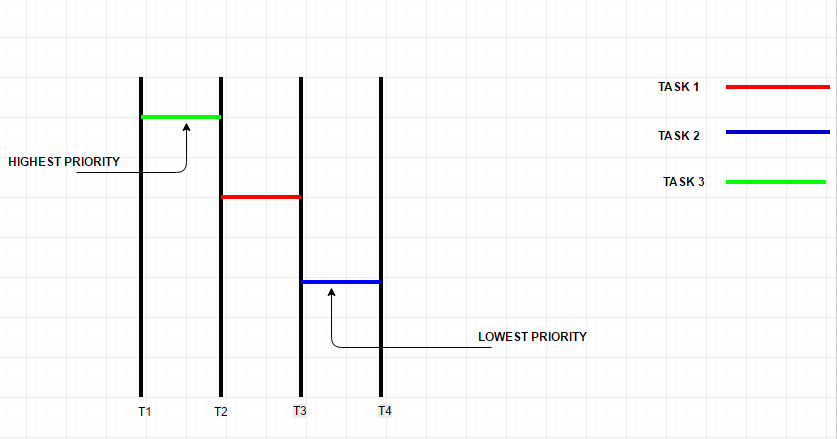
\includegraphics[width=10cm,height=5cm]{multitasking_states.PNG}
\caption{Multitasking state diagram}
\end{figure}

\item \textbf{\href{https://github.com/eYSIP-2016/RTOS_LPC2148/tree/master/Semaphore_Binary}
{Binary Semaphore:}}Semaphores are used for task synchronization,the above code illustrates how two tasks are ensured resources(i.e control of motors) with the help of Binary semaphore.
\begin{figure}[h]
\centering
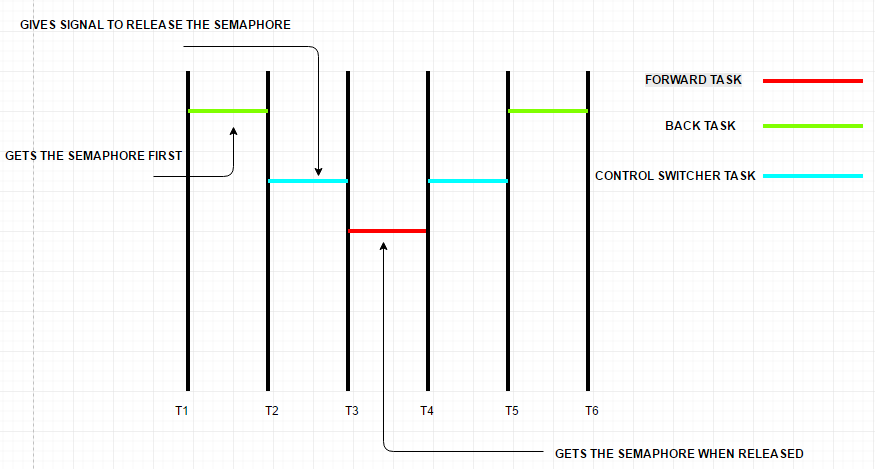
\includegraphics[width=10cm,height=6cm]{Binary.PNG}
\caption{Binary Semaphore state diagram}
\end{figure}
\newpage
\item \textbf{\href{https://github.com/eYSIP-2016/RTOS_LPC2148/tree/master/Semaphore_mutex}{Mutex:}}Mutex are semaphores which ensure that the resources are only used by only one process. Once the task having the semaphore releases it after its use then only then the other tasks can get the semaphore. This is illustrated with an example which has output similar to that of Binary semaphore but has difference on implementation level.
\begin{figure}[h]
\centering
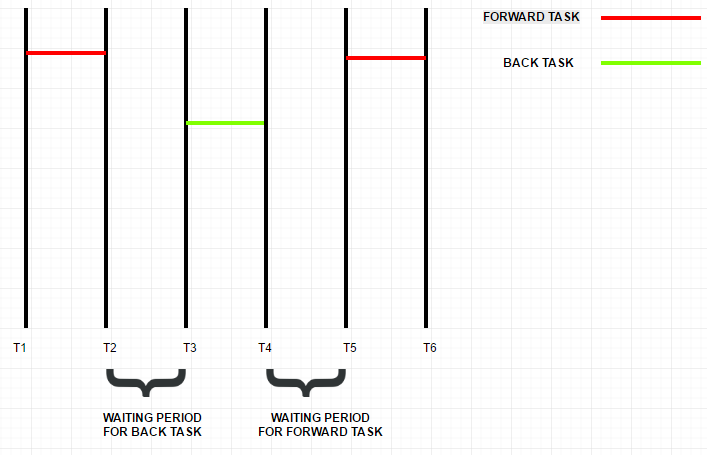
\includegraphics[width=10cm,height=7cm]{Mutex.PNG}
\caption{Mutex Semaphore state diagram}
\end{figure}

\\
\item \textbf{\href{https://github.com/eYSIP-2016/RTOS_LPC2148/tree/master/Semaphore_counting}{Counting Semaphore:}}The concept of counting semaphore has been illustrated by implementing a simulation of the dining philosophers problem.




\\
\item \textbf{\href{https://github.com/eYSIP-2016/RTOS_LPC2148/tree/master/MailBox}{MailBox :}}FreeRTOS doesn't directly support Mailbox but it can be implemented using TaskNotification.The message is communicated through predefined functions whose parameters can be varied to perform different operations on message,send different messages and manipulate existing or incoming message.
\\
\item \textbf{\href{https://github.com/eYSIP-2016/RTOS_LPC2148/tree/master/Queue}{Queues :}}Queues can be used to share data between multiple tasks,the data to be shared can be pushed into the queue and the tasks can receive data by receiving from the queue.FreeRTOS provides API's to make static queues,send data to queue and receive data from queue.A timeout period can also be mentioned for receiving/sending data to queue.
\begin{figure}[h]
\centering
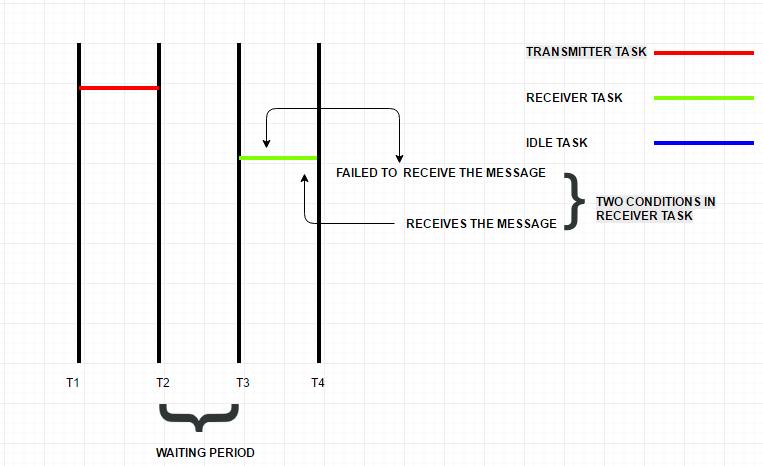
\includegraphics[width=10cm,height=5cm]{QUEUE.PNG}
\caption{Queue state diagram}
\end{figure}

\\
\item \textbf{\href{https://github.com/eYSIP-2016/RTOS_LPC2148/tree/master/ContextSwitching}{Context Switching:}}Context switching is saving the state of the process in the memory when another process is allocated the processor time.This has been illustrated with switching between tasks of different priorities.
\begin{figure}[h]
\centering
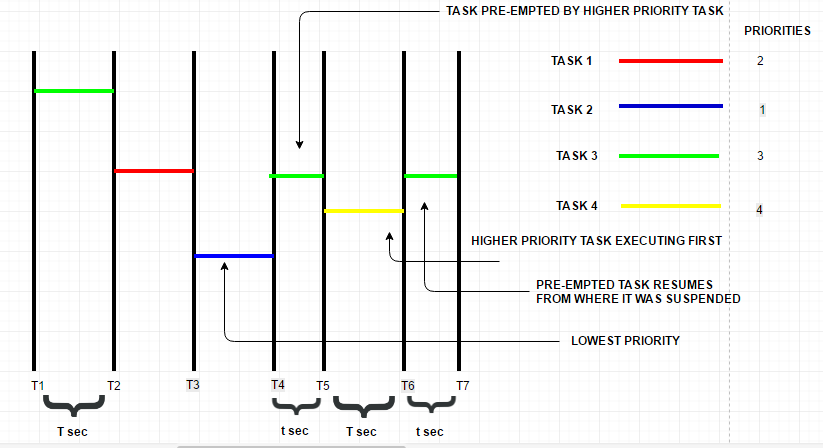
\includegraphics[width=10cm,height=7cm]{CONTEXTSWITCHING.PNG}
\caption{Context Switching}
\end{figure}
\newpage


\item \textbf{\href{https://github.com/eYSIP-2016/RTOS_LPC2148/tree/master/State_collector}{State collection :}}This code consists of a Task which stores data in a variable and another which sends it through UART,using these "tasks" sensor values can be obtained for later use.
\begin{figure}[h]
\centering
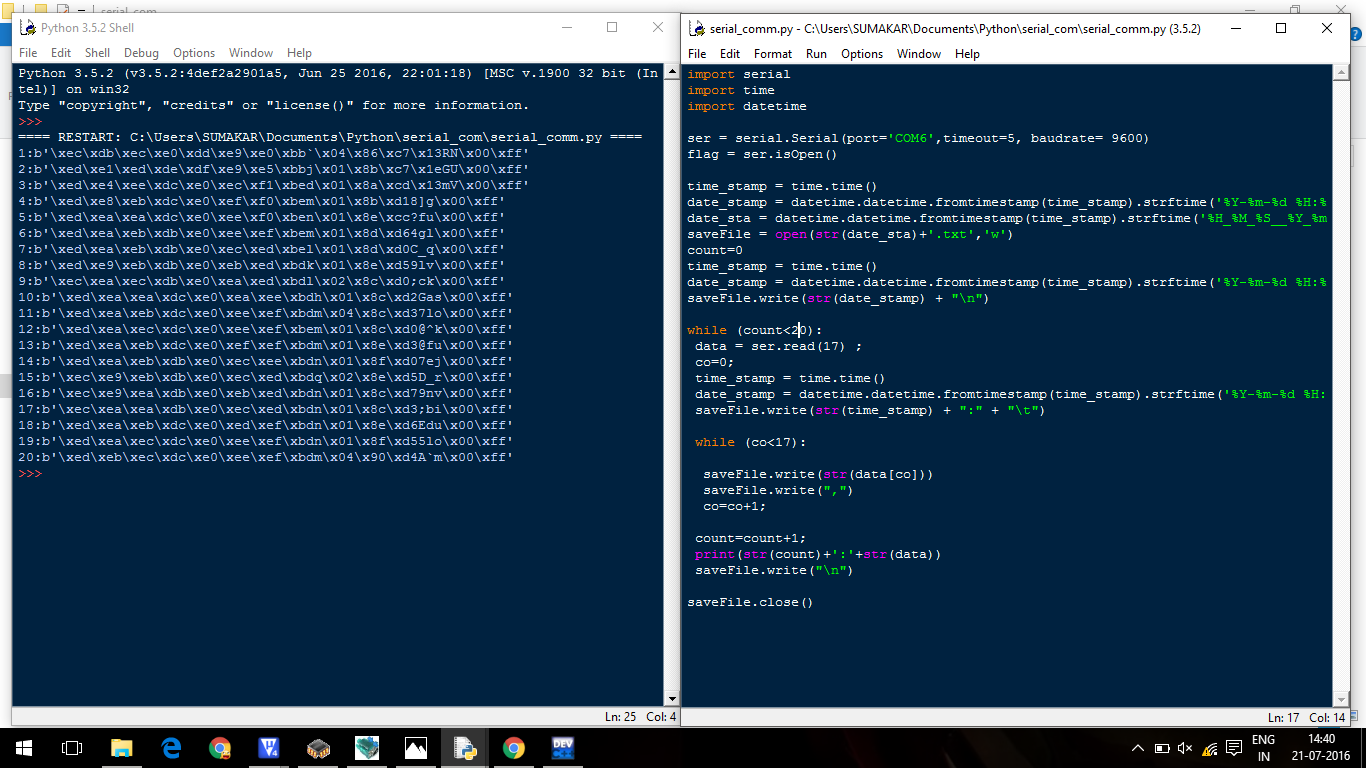
\includegraphics[width=15cm,height=10cm]{Statecollection.png}
\caption{State collection}
\end{figure}
\begin{figure}[h]
\centering
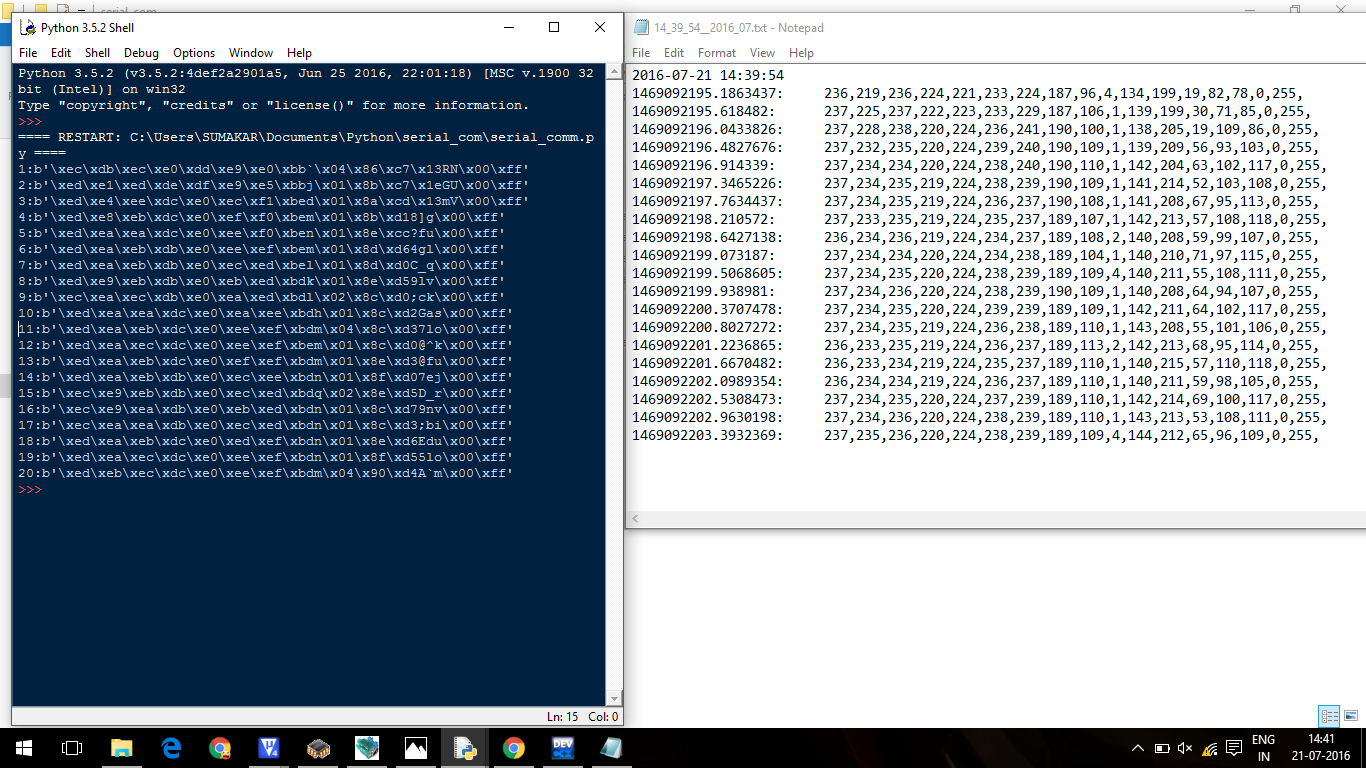
\includegraphics[width=15cm,height=10cm]{Statecollection2.png}
\caption{State collection}
\end{figure}

\newpage

\\
\item \textbf{\href{https://github.com/eYSIP-2016/RTOS_LPC2148/tree/master/serial_com}{Serial to file:}}This python script can be used to read the state collection data from a COM port(via serial communication or Xbee) and save the obtained data into a text file(comma seperated values with time stamp).
\\
\item \textbf{\href{https://github.com/eYSIP-2016/RTOS_LPC2148/tree/master/SPI_ADC}{SPI1 :}}This code was an improvement of an already existing code.This code prints the values of sensors connected to slave(2 Atmega 8 uC) on an LCD display.
\\
\item \textbf{\href{https://github.com/eYSIP-2016/RTOS_LPC2148/tree/master/Collision\%20avoidance}{Collision Avoidance:}}With the help of this code we are trying to illustrate the difference between RTOS and 'normal C'.The difference in the behaviour of the robot can be observed for a similar logic for different implementation.
%\item \textbf{\href{}{}}
\end{itemize}

%Brief explanation of various parts of code 
\newpage
%\section{Use and Demo}
%Final Setup Image

%User Instruction for demonstration

%\href{http://www.youtube.com}{Youtube Link} of demonstration video 
%\newpage
\section{Future Work}
%What can be done to take this work ahead in future as projects.
RTOS is something which is useful only when required therefore we think developing modules for LPC2148 with support to RTOS would be a better direction,here are some of the suggestions/ideas we were trying to work upon.
\begin{enumerate}
    \item Making FireBird more acessible 
    \begin{itemize}
        \item FireBlocks for LPC2148 and android support for the same.
        \\
        \item Interfacing FireBird to Smartphone via USB to directly program it by transferring the .bin file.
    \end{itemize}
    \\
    \item Interfacing Lower resolution camera modules like ov7670 to perform/learn basic level image processing.
    
    \item Improvements in state collection.
    \begin{itemize}
    \item A SD card module can be added to store state data in the SD card instead of EEPROM or transmitting via Xbee.
    \\
    \item Interfacing a Wifi module with LPC2148 to log data directly on servers.   
    \\
    \item Encoding the data in the bot itself before transmission.
    \end{itemize}
    
    \item Improvements in Collision avoidance.
    \begin{itemize}
    \item Using UltraSonic sensors to detect obstacles from far and calculate its course of action/velocity etc.
    \end{itemize}}
\end{enumerate}
\newpage
\section{Bug report and Challenges}
%Any issues in code and hardware.
\large{\textbf{Bug report}}
\begin{itemize}
  \item The UART FIFO of LPC2148 is of 16 Bytes ,if more than 16 bytes of data is sent at the same time data loss may occur.
  \\
  %\item Interrupts support is not available therefore position encoders couldn't be used.
  \item Data obtained in python script is not validated and is directly stored into the files so loss of data wouldn't be countered.
  \\
  \item In the collision avoidance Experiment if the obstacle is in its blind spot the bot would collide.
  \\
  \item FreeRTOS provides a common header file for all LPC21xx microcontrollers, using it had given us warnings/errors we had replaced the contents of lpc21xx.h file with that of lpc214x.h .
    \end{itemize}
\newline
  \large{\textbf{Challenges}}
  \begin{itemize}
  
  \item Learning how to port FreeRTOS.
  \item Getting Sensor data from SPI1.
  \item Understanding the implementation level difference between Binary semaphore and Mutex.
  \item IR's connected to Master were giving incorrect values we instead used Sharp sensors.
  \item Bringing out an example which can illustrate the advantage of using RTOS.
  \end{itemize}
 \newline 
%Any failure or challenges faced during project
 \large{\textbf{Failures :}}
 \begin{itemize}
  
 \item Unable to interface with smart phone.
 
\end{itemize}

\end{document}

